%%
% Please see https://bitbucket.org/rivanvx/beamer/wiki/Home for obtaining beamer.
%%
\documentclass{beamer}
\usepackage{url}
\usepackage{amsmath}
\usepackage{amsfonts,amssymb,amsthm,cite,float,graphicx}
\usepackage{physics}
\usepackage{graphicx}
\usepackage{mathtools}
\usepackage{float}

%new math symbols taking no arguments
\newcommand\0{\mathbf{0}}
\newcommand\CC{\mathbb{C}}
\newcommand\FF{\mathbb{F}}
\newcommand\NN{\mathbb{N}}
\newcommand\QQ{\mathbb{Q}}
\newcommand\RR{\mathbb{R}}
\newcommand\ZZ{\mathbb{Z}}
\newcommand\bb{\mathbf{b}}
\newcommand\kk{\Bbbk}
\newcommand\mm{\mathfrak{m}}
\newcommand\pp{\mathfrak{p}}
\newcommand\xx{\mathbf{x}}
\newcommand\yy{\mathbf{y}}
\newcommand\GL{\mathit{GL}}
\newcommand\into{\hookrightarrow}
\newcommand\nsub{\trianglelefteq}
\newcommand\onto{\twoheadrightarrow}
\newcommand\minus{\smallsetminus}
\newcommand\goesto{\rightsquigarrow}
\newcommand\nsubneq{\vartriangleleft}

\AtBeginSection[]
{
  \begin{frame}
    \frametitle{Table of Contents}
    \tableofcontents[currentsection]
  \end{frame}
}

\title{Bosonic Codes in 5 Minutes}
\author[Sbahi] % (optional, for multiple authors)
{Faris Sbahi}
\date{10/28/18}
\subject{Physics}

\begin{document}

\maketitle

\section{Introduction}

\begin{frame}
\frametitle{Bosonic Codes}
\begin{itemize}
\item Encode information in the space corresponding to the occupation (photon) number of a harmonic oscillator
\item Characterize by
\begin{enumerate}
\item Fock/number states $\{\ket{n}\}^\infty_{n=0}$
\item position and momentum eigenstates $\{\ket{x}\}_{x\in\RR}, \{\ket{p}\}_{p\in\RR}$
\item coherent states $\{\ket{\alpha}\}_{\alpha\in S}$ for some $S$
\end{enumerate}
\item Photons are prone to "loss" (action by $a$). So, we can focus on correcting these errors.
\item Photon-photon interactions are extremely weak
\end{itemize}
\end{frame}

\begin{frame}
\frametitle{Harmonic Oscillator Review}
\begin{itemize}
\item non-Hermitian creation/annihilation operators: $a^\dag, a$
\item ${{\begin{aligned}a^{\dagger }|n\rangle &={\sqrt {n+1}}|n+1\rangle, \qquad a|n\rangle &={\sqrt {n}}|n-1\rangle\end{aligned}}}$
\item $b = a^{\dag }a, \qquad n\ket{n} = n\ket{n} $
\item $[a,a^{\dag }]=1,\qquad [n,a^{\dag }]=a^{\dag },\qquad [n,a]=-a,$
\pause
\item Coherent states: eigenfunctions of annihilation operator 

$$
|\alpha\rangle =e^{-{|\alpha|^2\over2}}\sum_{n=0}^{\infty}{\alpha^n\over\sqrt{n!}}|n\rangle =e^{-{|\alpha|^2\over2}}e^{\alpha\hat a^\dagger}|0\rangle ~,
$$

\item Note: notation ${\displaystyle |\alpha \rangle }$  does not refer to a Fock/number state.

\item Expression ${\displaystyle |\alpha \rangle } $  with $\alpha = 2$ represents a Poisson distribution of number states ${\displaystyle |n\rangle }$  with a mean photon number of two. Think Poisson arrival process, but with photons.
\end{itemize}
\end{frame}


\begin{frame}
\frametitle{Hopeful approach: Apply Ken's course directly}	
\begin{itemize}
\item Simple encoding of $M$ qubits: $2^M$ Fock states cover photon numbers $0, 1, . . . , (2^{M - 1})$.
\item Use binary representation: $\ket{n} = \ket{b_{M-1} b_{M-2} \cdots b_0 }$
\item The $j$th binary digit represents the eigenvalue $(1 + Z_j)/2$ for the corresponding physical qubit 
\item E.g., $n=8$: $\ket{1000}$
\pause
\item Photon loss occurs, $a : \ket{1000} \mapsto \ket{0111}$
\item QEC schemes based on models of independent single qubit errors cannot be easily transferred to this problem
\item Luckily, the stabilizer formalism provides useful intuition for codes we'll discuss
\end{itemize}
\end{frame}

\begin{frame}
\frametitle{Knill-Laflamme conditions}
\begin{itemize}
\item Quantum Error Correction criteria
\item Find two logical code words $\ket{W_\sigma}$, where $\sigma = \uparrow, \downarrow$ s.t. 

$$\bra{W_\sigma} E_l^\dag E_k \ket{W_\sigma} = \alpha_{l, k} \delta_{\sigma, \sigma'}$$

 for all single, independent errors $E_{l,k} \in \mathcal{E}$
 \item Also, require $\alpha_{l,k}$ are entries of a Hermitian matrix and independent of the logical words.	
\end{itemize}
\end{frame}


\section{Single Mode Codes}

\begin{frame}
\frametitle{Simple Code}
\begin{itemize}
\item Reminder from quantum optics: mode = frequency + spatial distribution + polarization
\item Protect against $\mathcal{E} = \{ I,a\}$
\item $\ket{W_\uparrow} = \frac{\ket{0} + \ket{4}}{2}$, $\ket{W_\downarrow} = \ket{2}$
\pause
\item Hence, $\ket{E_1} = \ket{3}$ and $\ket{E_2} = \ket{1}$
\item Distinguish states by measuring number and checking mod 4
\pause
\item Same mean photon number i.e. $\bra{W_\sigma} n \ket{W_\sigma} = 2$
\begin{itemize}
\item So, $a : \alpha\ket{W_\uparrow} + \beta\ket{W_\downarrow} \mapsto \alpha \ket{E_1} + \beta \ket{E_2}$ (no deformation)
\end{itemize}
\pause
\item Generalize
\begin{itemize}
\item Greater spacing between states: can detect higher order loss errors or alternatively gain errors
\item Action by $n$ "dephases" (see how it can shift relative phases?). This leads to a superposition of codewords and error words. Project onto word basis to recover (efficient).
\end{itemize}
\end{itemize}
\end{frame}

\begin{frame}
\frametitle{Binomial Codes}
\begin{itemize}
\item Protect against $\mathcal{E} = \{I, a, a^2, \cdots, a^L, a^\dag, \cdots, (a^\dag)^G, N, \cdots, N^D \}$
\item Consider

$$
\ket{W_{\uparrow / \downarrow}} = \frac{1}{\sqrt{2^N}} \sum_{ p\text{ even/odd}}^{[0, N+1]} \sqrt{\binom{N+1}{ p }} \ket{p(S+1)}
$$

with $S = L+G$, $N = \max\{L, G, 2D\}$.

\item Now, trust me that it works similarly to before!
\pause
\item Mean photon numbers equal (no deformation) and QEC condition holds
\item Can be shown by writing difference in $l$th moment of photon number of codewords as $l$th derivative of $(1+x)^{N+1}\vert_{x=-1}$ with $l \leq \max\{L, G\}$ up to a factor
\item Measure photon number mod $S+1$
\end{itemize}
\end{frame}

\begin{frame}
\frametitle{Cat Codes}
\begin{itemize}
\item Superposition of well-separated coherent states ("legs")
\item $2(L+1)$ legs protects $L$ photon losses. Compare to binomial code with $S=L$
\item E.g. $L=1$

$$
\ket{C^\alpha_{\uparrow/\downarrow}} = \ket{\alpha} \pm \ket{i \alpha} + \ket{-\alpha} \pm \ket{-i \alpha} 
$$

up to a normalization factor.
\item As $\alpha \rightarrow \infty$, $\bra{C^\alpha_{\uparrow}} N^p \ket{C^\alpha_{\uparrow}} = \bra{C^\alpha_{\downarrow}} N^p \ket{C^\alpha_{\downarrow}}$ so potentially immune from unlimited order dephasing
\item Remember: distributed as Poisson and for large $N$, Binomial and Poisson approach normal distribution
\item Loss takes coherent states to coherent states! Can measure mod $S+1$ again to determine whether jump occurred. Do we do anything, if not?
\end{itemize}
	
\end{frame}

\begin{frame}
\frametitle{GKP Codes}
\begin{itemize}
\item Use the continuous basis of non-normalizable eigenstates of the position operator $x$	
\item Not enough time!
\item Quantum analoge of frequency combs
\item Key: protect against displacement errors $D_\alpha = \exp{\alpha a^\dag  - \alpha* a}$, not loss errors explicitly
\end{itemize}
	
\end{frame}


\section{Error Models and Performance}

\begin{frame}
\frametitle{Error Models}
\begin{itemize}
\item Some reminders
\item Photons are prone to loss
\item Photon-photon interactions are extremely weak
\item Hence, bosonic QEC codes focus on correcting photon-loss errors using very limited forms of photon-photon interactions
\end{itemize}
\end{frame}

\begin{frame}
\frametitle{Pure Loss Bosonic Channel}
\begin{itemize}
\item Assume encoding, recovery, and decoding are perfect
\item Lossy channel $N = \exp(\kappa t D)$ with superoperator $D(\cdot) = a a^\dag - 1/2 \{ n , \cdot \}$ with $\kappa$ as the excitation loss rate and time interval $t$
\item Kraus operators
$$
E_l = (\frac{\gamma}{1-\gamma})^{l / 2} \frac{a^l}{\sqrt{l!}}(1 - \gamma)^{n / 2}
$$
with $\gamma = 1 - \exp(- \kappa t)$

\item Channel does not contain identity as a Kraus operator for $\gamma \neq 0$ due to aforementioned damping/back-action
\item VV Albert considers "channel fidelity", $F_\mathcal{E}$, which is the overlap between the initial state and the final state when considering an initial Bell state such that only the first qubit is acted on by the channel
\item Optimal recovery for each code is computable via a semi-definite program
\end{itemize}
\end{frame}

\begin{frame}
\frametitle{Channel Fidelity}
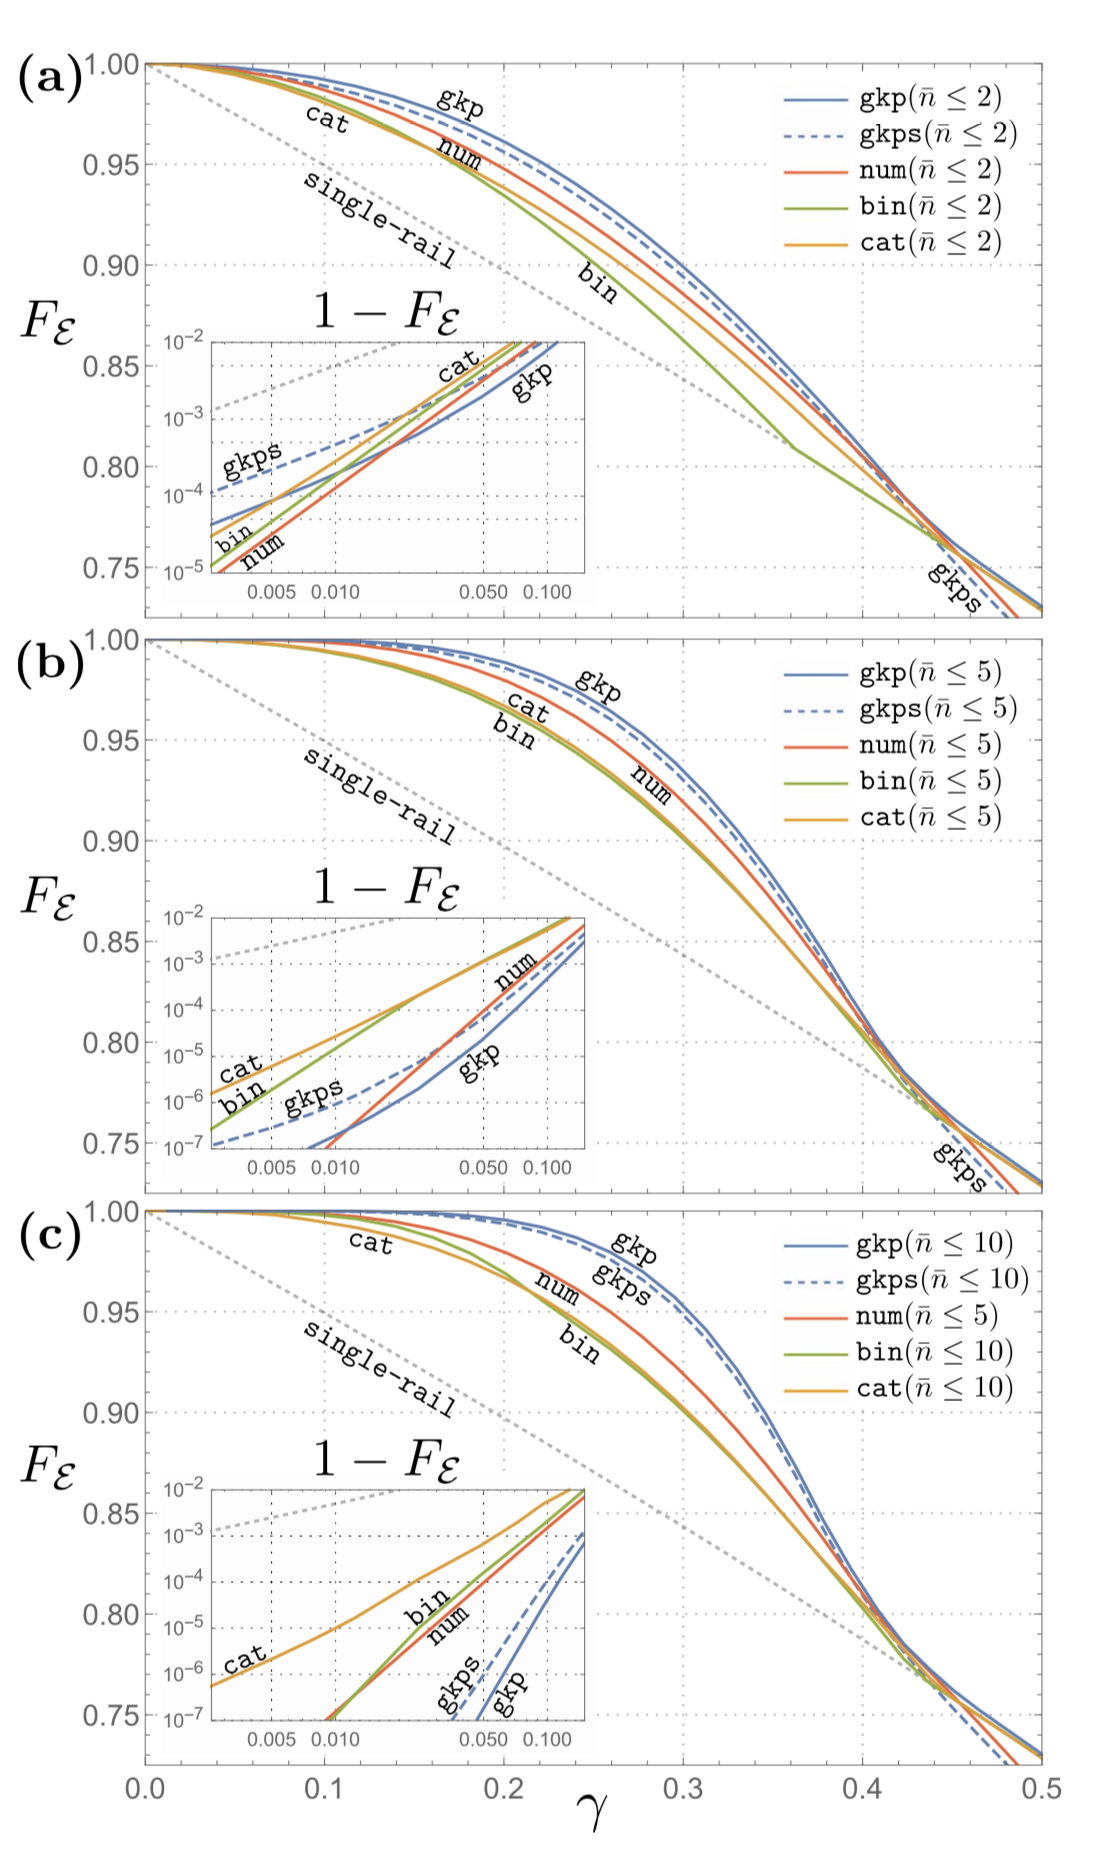
\includegraphics[width=\linewidth,height=0.9\textheight,keepaspectratio]{fidelity.png}
\end{frame}


\section{Multi-Mode Extensions}

\begin{frame}
\frametitle{Multi-Mode Extensions}
\begin{itemize}
\item Pair-cat codes
\item $\chi^{(2)}$ codes
\item noon codes
\item Experimentally relevant advantages over single-mode codes 
\item Correct more errors
\end{itemize}
\end{frame}

\begin{frame}
	\frametitle{Multi-Mode Extensions: Binomial Codes}
	\begin{itemize}
	\item To create more useful quantum superpositions of Fock states which can store quantum information, it is necessary to couple the bosonic mode to a non-linear element, e.g., a superconducting qubit, a trapped ion, or a Rydberg atom
		\item $\chi(2)$ code uses $O(n)$ instead of $O(n^2)$ qubits that previous two mode codes had used to correct $m$ loss/gain/dephasing errors (Niu)
		\item Inspired by cat code, but uses lower order non-linearity
	\end{itemize}

	
\end{frame}

\begin{frame}
	\frametitle{Multi-Mode Extensions: Cat Codes}
	\begin{itemize}
		\item Pair-cat codes (VV Albert)
		\item Reduction in order of nonlinearity required for physical realization (as with $\chi(2)$)
		\item With ordinary cat codes and current technology, the number parity syndrome makes it difficult to realize simultaneous discrete (usually for loss) and continuous error correction  (usually for dephasing)
	\end{itemize}

	
\end{frame}


\end{document}
